\documentclass{acm_proc_article-sp}

\begin{document}

\title{Protecting Browsers from Cross-Origin CSS Attacks}

\numberofauthors{3}
\author{
\alignauthor
Chris Evans\\
      \affaddr{Google}\\
      \affaddr{cevans@google.com}
\alignauthor
Lin-Shung Huang\\
      \affaddr{Carnegie Mellon University}\\
      \affaddr{linshung.huang@sv.cmu.edu}
\alignauthor
Collin Jackson\\
      \affaddr{Carnegie Mellon University}\\
      \affaddr{collin.jackson@sv.cmu.edu}
}

\maketitle
\begin{abstract}
The cross-origin CSS attack is a newly exploited browser vulnerability that allows the attacker to steal a user's secret content on an honest web site from a different domain. In this paper, we expose the cross-origin CSS attack, which involves cross-origin style sheet loading and CSS property string injection to steal cross-origin data. This attack is constructed upon the lenient MIME type requirement and lax CSS parsing in modern browsers. We propose browsers to implement a stricter cross-orign CSS checking which can provide robust defense for cross-origin CSS attacks while addressing web site compatibility concerns. We detail other client-side and server-side mitigation techniques and find shortcomings with each technique. Our proposal has been adoped by Google Chrome, Safari and Opera.
\end{abstract}

\category{K.6.5}{Management of Computing and Information Systems}{Security and Protection}

\terms{Security}

\keywords{CSS, MIME, Same-Origin Policy}

\section{Introduction}
(This is the introduction.)

browser quirks/strict modes

Content sniffing XSS\cite{securecontentsniffing}

JavaScript hijacking\cite{jshijacking}

In the cross-origin CSS attack, the attacker injects CSS strings into the target domain that contains the secret content, instructs the victim's browser to import and parse the target document as a style sheet, and then exports the secret string from the computed style properties to the attacker.

\section{Threat Model}
We define a precise threat model, the web attacker, for reasoning the cross-origin CSS attack. We assume that the attacker's goal is to steal a victim user's secret content on an honest web site from another domain.

\subsection{Web Attacker}
A web attacker is a malicious principal who owns a domain name, e.g. attacker.com, and operates a web server. To study the browser's defense mechanisms, we assume that the victim's browser renders content from the attacker's web site. In addition, the web attacker is given the ability to inject semi-arbitrary strings into the target domain.

\begin{itemize}

\item{Attacker Abilities:}
The web attacker can send and receive network messages over network protocols of the attacker's choice, but only from its own machines. Typically, the web attacker operates at least one machine as an HTTP server, which we refer to as \texttt{attacker.com}. The web attacker has no control over the victim's network connections. In particular, the web attacker cannot eavesdrop on unencrypted connections and steal session identifiers to hijack the victim's authenticated user session. Neither can the web attacker spoof network frames and impersonate another user to an honest web site.

\item{Victim Behavior:}
We assume that the victim visits the attacker's web site with a popular browser. In practice, this assumption can be supported by several techniques for attacking users, e.g. buying web advertisements or sending bulk e-mail to encourage visitors. By visiting \texttt{attacker.com}, the attacker can instruct the victim's browser to fetch external style sheets and also export data to remote servers. As long as the victim's session with an honest web site haven't expired, the attacker can instruct the victim's browser to issue requests with the victim's cookies.

\item{Target Behavior:}
We assume that the attacker can inject semi-arbitrary strings into a target domain that contains the secret content, which we refer to as \texttt{target.com}. We define the term semi-arbitrary strings as a subset of strings that may conform to CSS syntax to differentiate from fully arbitrary strings that may also conform to HTML syntax. The ability of injecting CSS strings is considered weaker than injecting HTML strings into the target domain, as in common XSS attacks, because scripts may be detected and blocked by client-side XSS filters. In practice, there are various methods to inject strings into the target domain, e.g. reflection of user-controlled strings or via URL parameters.

\end{itemize}

There are a number of related threats that we do not consider in this paper, such as phishing, DNS rebinding, and XSS.
(more description...?)
The web attacker is incapable of installing malicious software on the victim's machine, otherwise, the malware could replace the browser and bypass any browser-based defenses.

\section{Attacks}
In this section, we study cross-origin CSS attacks. First, we provide some background information. Next, we introduce cross-origin CSS attacks. Then, we discuss the restrictions for constructing this attack and suggest general areas that are exploitable. Finally, we demonstrate an attack against a popular web site as our proof of concept.

\subsection{Background}
In this section, we provide background information about Cascading Style Sheets (CSS), the same-origin policy (SOP), and MIME types.

\subsubsection{Cascading Style Sheets}
Cascading Style Sheets\cite{css} is a mechanism that lets web developers control the visual appearance of web documents using style sheet language. The design of CSS enables separation of document content from the visual appearance, including layouts, colors, and fonts. This allows web sites to adjusting its appearance, e.g. switching on-screen views to printable views, without requiring modifications to the document. Furthermore, documents are allowed to import external style sheets and let third parties to control a subset of the CSS rules. This feature allows web sites to share style sheets across a number of documents.

\paragraph{Lax Parsing}
In modern browsers, the CSS parser is actually very lax. The CSS parser will skip over any amount of invalid syntax in the style sheet until it finds the next valid rule. This is unlike the JavaScript parser that will abort on the first syntax error. A lax CSS parser gives the browser better compatibility for supporting misconfigured web sites, but unfortunately opens opportunities to attackers and enables the cross-origin CSS attack in this paper.

(Chris' comment: I think they are intending to be forward-compatible with brand new CSS syntax too.
There is some small interpretation of invalid syntax: careful track seems to be kept regarding opened brackets. I think this includes { ( and [ -- but of course may be browser dependent. Any CSS injection point may have to close an arbitrary number of these brackets: of the correct type in the correct order!)

\subsubsection{Same-Origin Policy}
The same-origin policy\cite{mozillasameorigin} is the main security mechanism in modern browsers that provides isolation of contents between unrelated web sites. The same-origin policy restricts contents to access resources only from the same origin, which applies to scripting interactions, i.e. accessing the Document Object Model (DOM)\cite{dom} and transferring data using the \texttt{XMLHttpRequest} API. In SOP, the origin of a resource is defined as the protocol, host, and port. The same-origin policy does not apply to fetching and executing remote libraries, including scripts and style sheets, from a different origin.

\subsubsection{MIME Types}
The HTTP \texttt{Content-Type} header indicates the type of the content that is transmitted using Multipurpose Internet Mail Extensions (MIME)\cite{mime} types such as \texttt{text/plain} for plain text and \texttt{image/jpeg} for JPEG images. The line in the HTTP header typically looks like the following:
\begin{verbatim}
Content-Type: text/html; charset=utf-8
\end{verbatim}
Browsers use MIME types to determine how to handle the contents of HTTP responses. However, many misconfigured web servers fail to provide the correct MIME type of their resources. Due to web site compatibility concerns, modern browsers use content-sniffing algorithms\cite{securecontentsniffing} to guess the correct MIME type by inspecting the contents of HTTP responses.  Content-sniffing algorithms can override the provided MIME type and file extension of the document. Unfortunately, this quirk introduces chameleon documents, in which a document conforms to a benign file format (such as PDF) and contains malicious HTML.

\subsection{Cross-Origin CSS Attack}
In a cross-origin CSS attack, the attacker's main objective is to steal the victim's secret content on an honest web site from a different domain. The attacker is most likely interested in stealing any sensitive information in a cookie-authenticated web page, or preferably a secret CSRF token\cite{csrf} hidden in the document that may allow the attacker to hijack the user's session. In order to steal content from a different domain, the attacker leverages the fact that the browser's security policy allows external style sheets to be imported from cross-origin. The target document on an honest web site is injected such that portions of the document conform to CSS rules. As soon as the victim visits the attacker's malicious page, the cross-origin data is imported as style sheets and stolen. To describe the cross-origin CSS attack in detail, we decompose the attack into three main steps: CSS string injection, style sheet import, and data export.

\begin{figure}
\centering
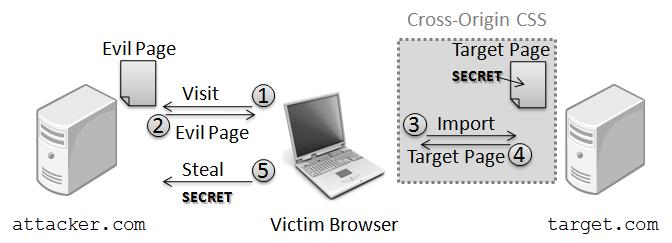
\includegraphics[width=\linewidth]{scenario.jpg}
\caption{Attack Scenario}
\end{figure}

\subsubsection{CSS String Injection}
Due to lenient MIME type requirement of CSS parsers, the attacker may fool the victim's browser into loading a carefully crafted non-CSS (e.g. HTML or XML) document as a valid style sheet resource. In practice, there are several methods that may allow a web attacker to inject strings into the target domain, e.g. reflection of user-controlled strings or via URL parameters. Normally, random text in a non-CSS document contains syntax errors to the CSS parser and would break the parsing. However, due to the overly lax CSS parsers in modern browsers, portions of a non-CSS document with valid CSS syntax can still be successfully parsed and recognized as style sheet rules.

To give an example of a CSS string injection, suppose that there is s sensitive content, represented with the string `SECRET', in an HTML document on an honest web site that the attacker wants to steal. Assuming that the attacker has sufficient influence over the web page to control the text preceding and succeeding the secret string, the CSS string injection can be constructed based on common CSS properties that corresponds to string values, i.e. \texttt{font-family}, \texttt{background-image}, and \texttt{list-style-image}. Given the ability to inject arbitrary strings into the target domain, the HTML document can be crafted to contain a CSS property \texttt{font-family} as the following:
\begin{verbatim}
Target document:
<HTML>..SECRET..</HTML>

After injection:
<HTML>..{} BODY { font-family: "SECRET" }..</HTML>
\end{verbatim}
The injected HTML document will appear to the CSS parser as containing a valid CSS rule. The fonts of the attacker's page will be styled with a font-family specified as the stolen string `SECRET'. Note that the seemingly redundant pair of brackets in the injection string re-syncs the CSS parser to make sure that the evil CSS rule parses properly. All the other non-CSS text in the document are skipped by the CSS parser, thus will not effect the parsing of the evil CSS rule. Once the crafted document is loaded, the attacker can easily steal the secret string from the computed \texttt{font-family} style of the attacker's page.

\begin{figure}
\centering
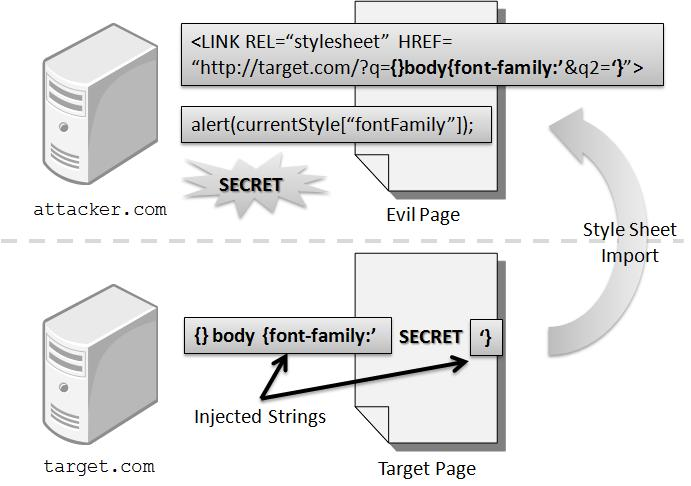
\includegraphics[width=\linewidth]{injection.jpg}
\caption{CSS String Injection}
\end{figure}

\subsubsection{Style Sheet Import?}
When the user visits \texttt{attacker.com}, the attacker's malicious page instructs the victim's browser to fetch and load the crafted document as a style sheet. In HTML specifications\cite{html}, documents can import external style sheets from remote servers by using the CSS \texttt{@import} notation, or using the link tag inside the head element as the following: .
\begin{verbatim}
<HTML>
<HEAD>
  <STYLE>
    @import url(http://target.com);
  </STYLE>
  <LINK REL="stylesheet" HREF="http://target.com">
</HEAD>
</HTML>
\end{verbatim}
\paragraph{Cookies}
The HTTP cookie mechanism enables web sites to authenticate clients and maintain client states, allowing web sites to not only serve static content but customize the content and appearance for each session user. According to the standards, the browser always sends the user's cookie when it loads any referenced style sheets, including cross-origin CSS. If a user was logged into the \texttt{target.com} while visiting the malicious page, the browser would send the user's authentication cookie on all requests to \texttt{target.com} and be considered as valid authenticated requests. This behavior exploits cookie-authenticated web sites and potentially leaks the user's sensitive information in the server's response. 

\subsubsection{Data Export?}
The final step for the attacker is to read the computed styles and export the secret content hidden in the style properties to the attacker. There are various methods to export data to other origins, in this specific attack we are interested in approaches where no user involvement is required. The cross-origin CSS attack is possible by just rendering one evil ad in the victim's browser. 

\paragraph{JavaScript}
One method is using JavaScript to access the loaded styles and then send the stolen data to attacker.com using the \texttt{XMLHttpRequest} API. All major browsers support using JavaScript to read computed styles even loaded from external style sheets through DOM access by calling the \texttt{window.getComputedStyle} method or retrieving the \texttt{currentStyle} object in Internet Explorer, given that the style name and property name is known by the attacker. WebKit-based browsers, i.e. Safari and Google Chrome, even surrendered the full CSS text of style sheets, including CSS rules loaded from cross-origin (without comments, thankfully). The attacker could read the raw text of cross-origin CSS via \texttt{document.styleSheets[].cssRules[].cssText} and also \texttt{window.getMatchedCSSRules().cssText}. This behavior violates the same-origin policy and potentially leaks data in pages with semi-valid CSS constructs. Other browsers only permit read access to the raw text of style sheets under restricted conditions. Internet Explorer allows access to cross-origin CSS raw text with \texttt{document.styleSheets[].cssText} only if the MIME type is correct. Firefox and Opera only allows access to CSS raw text for style sheets loaded from same-origin. Even if access to raw CSS text is blocked, the ability to read cross-origin loaded CSS styles is enough to construct serious attacks.

\begin{table}
\centering
\begin{tabular}{|c|c|c|c|c|c|} \hline
Methods&IE&FF&OP&Safari&Chrome\\ \hline
currentStyle&\checkmark&&\checkmark&&\\ \hline
getComputedStyle&&\checkmark&\checkmark&\checkmark&\checkmark\\ \hline
%rules[].style.cssText&\checkmark&&&\checkmark&\checkmark\\ \hline
cssRules[].cssText&&&&\checkmark&\checkmark\\
\hline\end{tabular}
\caption{Cross-Origin CSS DOM Vulnerabilities}
\end{table}

\paragraph{Background-image}
Another method is available to exploit users that have disabled JavaScript in their browsers by simply injecting the CSS property \texttt{background-image} string as the following:
\begin{verbatim}
<HTML>..{} BODY { background-image: url(http://att
acker.com/?SECRET); }..</HTML>
\end{verbatim}
Using this method, the secret string is appended to the path or query string of the attacker's server URL. Therefore, the background of the attacker's page will be styled with a background image loaded from an URL, the path of which contains stolen data. One important characteristic of the CSS property \texttt{background-image}, which is an URL, is that it will be automatically fetched even if JavaScript is turned off. The stolen data is then harvested by the attacker from their web server logs.

\subsection{General Restrictions}
The cross-origin CSS attack is less serious than it could be, because there are a few restrictions of cross-origin data which can be stolen.

\subsubsection{Sufficient Injection Points}
The first and most crucial step of the cross-origin CSS attack is to contain the secret data into a CSS property string. In order for the CSS parser to properly parse the evil CSS rule, certain symbols must be inserted at the beginning and at the end of the stolen string. In general, the attacker must have sufficient influence over the target document to control two injection points, pre-string and post-string, to insert the starting symbols and termination symbols, respectively. Typically, socially-related web sites are relatively more susceptible to this attack since the pages often contain user-controlled strings such as comments on photos. For some web sites, a second injection is not required because the termination symbols happens to exist later in the document. This is possible since the termination symbols can be as short as just a quotation mark and an ending bracket. 

\subsubsection{Avoid Character Escapes}
In CSS specifications\cite{css}, strings can either be written with double quotes or with single quotes. Double quotes cannot occur inside double quotes, analogously for single quotes. Therefore, the attacker has the choice to inject either single or double quotes depending on the occurrence of quotes in the secret data. In a context where both quotes are escaped, it becomes more difficult to inject a CSS string. However, a variation of the attack  can bypass this restriction by injecting the CSS property \texttt{background-image}. For the \texttt{background-image} property, the URL value is written with the functional notation \texttt{url()}, which does not require the use of single or double quotes around the URL string itself. The CSS specification does define that certain characters must be escaped in an unquoted URL, e.g. parentheses, commas, white spaces, single quotes and double quotes. However, in Internet Explorer, the CSS parser does not require any of these characters to be escaped in an unquoted URL and will parse until it encounters a closing parentheses and a semicolon.

\paragraph{Force UTF-7}
The requirement for quotes to not get escaped can sometimes be bypassed in browsers that support UTF-7 encoding, including Firefox and Safari. If the target web sites fails to specify a character set in the HTTP \texttt{Content-Type} header, the attacker's malicious page can force the remote resource to be parsed as UTF-7 encoding as the following:
\begin{verbatim}
<LINK REL="stylesheet" HREF="http://target.com" 
CHARSET="utf-7">
\end{verbatim}
By forcing UTF7, either a single or double quote may be injected by rendering it in the UTF-7 character set, i.e. `\texttt{+ACc-}' for single quote and `\texttt{+ACI-}' for double quote. This will cause the injection to survive any output escaping of the web application. A significant number of web sites actually do not specify character sets in their HTTP responses (We found that 22 out of the top 100 web sites ranked by Alexa\cite{alexa} did not specify character sets). Some web sites specify the \texttt{Content-Type} information using meta tags with the \texttt{http-equiv} attribute in the HTML head element as the following:
\begin{verbatim}
<META HTTP-EQUIV="Content-Type" CONTENT="text/html; 
charset=utf-8">
\end{verbatim}
Browsers may use meta tags to refine the information provided by the actual headers, but can also ignore it. If a document declares a character set in a meta tag but not in the response header, the referring page can override the character set with the \texttt{charset} attribute in the parent link tag. Thus, using the equivalent HTTP header to specify the MIME type and character set is always recommended.

\subsubsection{Avoid Newlines}
In CSS, a string cannot directly contain a newline. To include a newline in a string, the line feed character must be escaped. Therefore, another barrier of this attack is that any un-escaped newline in the stolen string will break the CSS parsing. This is a very common condition in many web pages, which avoids potentially serious attacks. However, many rich-functionality web sites are often exploitable due to serving subtle cookie-authenticated URLs with JSON or XML responses that commonly lack newlines. Some web sites even allow users to control the formatting of server responses, e.g. disable pretty printing, which may be extremely dangerous.
\paragraph{Internet Explorer}
Catastrophically, the CSS parser in the Internet Explorer accepts both newlines in CSS strings and newlines in unquoted URL strings, regardless of whether escaped or not. Unfortunately, even a fully-patched browser can expose its users to a cross-origin CSS data theft and potentially serious session hijacking.

\subsection{Concrete Attacks}
In this section we illustrate the cross-origin CSS attack with an example.

?? mixi.jp post\_key theft\cite{cssxss}

Example: Yahoo! Mail

\section{Defenses}
In this section, we describe the defenses against cross-orgin CSS attacks. First, we propose to stricten the requirements for loading cross-origin CSS references. Next, we present an evaluation of web site compatibility for our proposal. Then, we state the progress of adoption for our proposal in major browsers. Finally, we discuss the shortcomings of other defensive approaches, including client-side and server-side mitigations.

\subsection{Proposal: Cross-Origin CSS Checking}
To prevent cross-origin CSS attacks, we propose that browsers should apply stricter checking when loading cross-origin CSS files. Our initial approach is to enforce strict MIME type checking for loading cross-origin CSS files, referred as the strict approach. We devise a conservative approach with additional CSS parser testing that maximizes web site compatibility while blocking most attacks.

\subsubsection{Strict Approach}
In the cross-origin CSS attack, the attacker's malicious web page confuses the victim's browser to parse an injected non-CSS document as a style sheet. If browsers strictly required external style sheets to specify the correct MIME type, which is \texttt{text/css}, the malicious web page would not be able to load any crafted document. One effective solution is to let browsers always check the MIME type of external CSS references and block any CSS load with an invalid MIME type. When strict MIME type checking is enforced, at least for cross-origin CSS loads (if not globally), browsers would be able to protect target non-CSS docuemnts from being stolen.

The major concern of the strict approach is that any misconfigured cross-origin resources that fail to provide valid MIME types would be blocked. Strict MIME type checking relies on web developers to correctly deploy their web sites and provide valid MIME types. Unless every web developer properly configures their servers to send the correct \texttt{Content-Type} response header, the strict approach will inevitably introduce false positives and cause CSS failure on web sites. Expectedly, browser vendors would tend to resist changes that would cause web site breakage and lose its users.

\paragraph{Strict Mode}
In fact, most modern browsers have a strict mode, or standard-compliant mode, that always require the correct MIME type when loading CSS files. However, strict modes are only triggered when the web developer declares a document type definition (DTD) in the referring document. Otherwise, the quirks mode, or compatibility mode, is used by default for better backward-compatibility. The strict mode option is not a mitigation to the cross-origin CSS attack because the attacker can simply avoid enabling strict mode by not declaring a doctype in their malicious documents. For web developers, it is always recommended to develop standard compliant web pages and add a \texttt{doctype} declaration at the beginning of the document to instruct the browser which version of the markup language you are using, as the following example:

\begin{verbatim}
<!DOCTYPE HTML PUBLIC "-//W3C//DTD HTML 4.01//EN"
 "http://www.w3.org/TR/html4/strict.dtd">
\end{verbatim}

\subsubsection{Conservative Approach}
To address web site compatibility concerns, we propose a conservative approach that blocks most attacks while tolerating MIME type misconfigurations. In order to reduce false positives in the strict MIME type approach, an additional level of checking is applied to cross-origin CSS loads that have invalid MIME types. When a valid MIME type is not provided, the browser will try to parse the cross-origin CSS but bailing on first syntax error. This simple parsing test helps to determine whether the imported CSS file is an injected target document. Therefore, the devised solution blocks a CSS load only when all of the following conditions are met:
\begin{itemize}
\item{The CSS load is a cross-origin.}
\item{The CSS load has an invalid MIME type. Valid MIME types are text/css, application/x-unknown-content-type, and empty.}
\item{The alleged CSS file does not start with a syntactically valid CSS construct.}
\end{itemize}
The above rules will block most cross-origin CSS attacks because the target documents that are not CSS files have headers that will cause a broken first CSS descriptor, e.g. HTML or XML headers. We also assume that a legitimate CSS file will unlikely have a syntax error at the beginning of the file and a broken MIME type, thus this heuristic should not break most existing sites. Only CSS files loaded from cross-origin with invalid MIME type that starts with malformed syntax is determined as an attacked document and rejected.

\subsubsection{Experiment}
To evaluate the compatibility of our proposed defense of stricter CSS loading, we conducted an experiment to measure how often web servers fail to provide the correct MIME type for CSS files and whether these CSS files are well-formed when loaded cross-origin.

\paragraph{Design}
To measure how often web servers fail to provide the correct MIME type for CSS files, we collected metrics by crawling the top 10,000 web sites ranked by Alexa\cite{alexa} and scanned through all of the style sheet resources in their home pages. We are interested in all CSS references including using HTML link tags and CSS \texttt{@import} directives. Furthermore, some web sites dynamically add CSS links using JavaScript while the page loads. To achieve a more thorough scan for these CSS references, we conducted our experiment to directly render these web pages with an instrumented WebKit browser while recording information of all CSS loads until the web page finishes loading.

\paragraph{Results}
From the top 10,000 web sites, we fetched a total of 27532 CSS references, including 22799 link tags and 4733 \texttt{@import} directives. These results do not include unreachable web sites nor unreachable CSS resources.

We found that as many as 172 CSS references on these popular sites did not provide the correct \texttt{Content-Type} response header. In most cases, we found that misconfigured servers provided the \texttt{text/html} MIME type for CSS files, which is for normal HTML documents. Some CSS files did not specify the \texttt{Content-Type} header in the response at all, thus had an empty MIME type. Our browser collected a list of various incorrect MIME types for CSS files, including \texttt{text/html}, \texttt{text/plain}, \texttt{text}, \texttt{application/octet-stream}, \texttt{application/x-pointplus}, \texttt{image/gif}, \texttt{Content-Type:text/css} and empty MIME type.

\begin{table}
\centering
\begin{tabular}{|c|c|c|} \hline
Content-Type&Percentage\\ \hline
text/html&87.78\%\\ \hline
Empty&7.56\%\\ \hline
text/plain&1.74\%\\ \hline
Other&2.90\%\\
\hline\end{tabular}
\caption{Misconfigured MIME Types for CSS}
\end{table}

According to the CSS parser of WebKit, our browser reported that 93 CSS files were mal-formed, which fail to have a syntactically valid CSS construct at the beginning to the file. There were three CSS files that were mal-formed and also have a broken MIME type, however none of these CSS files were cross-origin loads.

Within a total of 8352 cross-origin CSS loads, there were 40 of them that had a broken MIME type. Blocking these loads would cause CSS failure on 29 of the 10000 most popular web sites. However, we also observed that none of the cross-origin CSS files with broken MIME types were mal-formed.

%We ran a scan across the top 500,000 URLs looking for cross-origin loads of CSS with an invalid MIME type. Valid MIME types are defined as text/css, application/x-unknown-content-type, and empty. There were a total of 140 URLs detected that referenced cross-origin CSS with broken MIME types. We found that some of them were non-serious conditions, in which the site loaded a CSS file which is missing and redirected to a 404 html page. There were 60 URLs that would be considered as broken, including 13 with text/plain, 15 with text/html, 31 with application/css, and 1 with application/x-pointplus. If we apply the heuristics of the conservative approach, only one URL that served text/html MIME would fail to load, which was severely broken because it had valid CSS rules after a style tag.

\paragraph{Discussion}
Based on our results, deploying the strict approach would break CSS references on 0.29\% of the top web sites. Although not prominent, we expect that if any popular web site crashed due to stricter CSS loading, browser vendors would possibly resist to deploy this change in risk of losing its users.

In our observations, the conservative approach did not break any CSS references in the top 10000 web sites. The conservative approach is an appealing defense because it maximizes web site compatibility while blocking the cross-origin CSS attack.

Due to practical limitations of our automated scanning, all of the tested links were unauthenticated. It is possible that more sites will be broken after logging in.

\begin{figure}
\centering
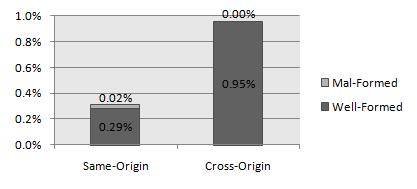
\includegraphics[width=\linewidth]{mime.jpg}
\caption{CSS Files with Incorrect MIME}
\end{figure}

\subsubsection{Adoption}
Our proposal requires no changes to existing web servers and only modifies the browser. We implemented the conservative approach of stricter CSS loading in a patch to WebKit, the open source web browser engine component integrated in Safari and Google Chrome. The WebKit patch was first deployed in Google Chrome 4.0.249.78, and also accepted in Safari 4.0.5. Note that the cross-origin CSS raw text leak is tightened by this patch because read access to cross-origin CSS raw text is limited to well-formed imports. Inspired by our WebKit patch, the exact same heuristic was adopted in Opera 10.10. Mozilla proposes (undetermined) to deploy a stricter MIME type checking for loading cross-origin CSS files in Firefox 3.6 quirks mode.

The interpretation of valid MIME types for cross-origin CSS on each browser slightly differs as shown in the table. In addition to the \texttt{text/css} MIME type, WebKit-based browsers accept files with \texttt{application/x-unknown-content-type} or empty MIME types, which also triggers the browser's content-sniffing algorithm in strict mode. Bogus represents incorrect MIME values that lack a slash.

\begin{table}
\centering
\caption{Always? Valid MIME Types for CSS}
\begin{tabular}{|c|c|c|c|c|} \hline
Content-Type&FF&OP&Safari&Chrome\\ \hline
text/css&\checkmark&\checkmark&\checkmark&\checkmark\\ \hline
application/x-&\checkmark&&\checkmark&\checkmark\\ 
unknown-content-type&&&&\\ \hline
Empty&\checkmark&&\checkmark&\checkmark\\ \hline
Bogus&\checkmark&&&\\ \hline
*/*&\checkmark&&& \\
\hline\end{tabular}
(should we include FF 3.7 dev results??)
\end{table}

\subsection{Other Approaches}
In this section, we further discuss some possible solutions to defend against the cross-origin CSS attack that we have considered. We argue that all of these approaches could either be circumvented with a variation of the attack, or would significantly reduce web site compatibility.

\subsubsection{Client-side Defenses}
There are other approaches that can be deployed in browsers without modifying web servers including globally blocking cookies, tightening DOM access and enforce stricter CSS parsing.

\paragraph{Block Cookies:}
Browsers give users the option of disabling cookies and always send anonymous requests, thus can prevent web attackers from stealing content on any cookie-authenticated URLs. However, disabling cookies would literally break a huge amount of sites that requires logging in. A more conservative approach would be to prevent sending cookies when sending requests for cross-origin CSS. However, that would still crash legitimate web sites that provide user-specific styles using external style sheets.

\paragraph{Restrict DOM Access:}
The same-origin policy for DOM access restricts the ability for JavaScript to access DOM properties and methods across domains. To prevent the cross-origin CSS attack, browsers should cautiously block DOM access to style sheets loaded from cross-origin, at least when the CSS file is malformed or has incorrect MIME type. However, all major browsers grant read access to computed styles loaded from cross-origin using either \texttt{window.getComputedStyle} or \texttt{currentStyle}, violating the same-origin policy. Even if browsers restricted the read access to computed styles for cross-origin loads, the attacker could bypass this limitation with \texttt{background-image} property injection that could automatically export data in requests to cross-origin servers.

\paragraph{Stricter CSS Parsing:}
CSS parsers are tolerant of syntax errors and will resume parsing after syntax errors. The cross-origin CSS attack could be mitigated if the browser's CSS parser always crashed hard on the first syntax error, like JavaScript parsers. However, this approach would require all web developers to strictly write well formed CSS, and would immediately break many existing web sites.

\subsubsection{Server-side Mitigations}
There are also some approaches that can be applied on web servers without requiring changes to current browsers, including using newlines, escaping characters and not using cookies.

\paragraph{Newlines}
In CSS specification, strings cannot directly contain newlines. Thus, a mitigation to the cross-origin CSS attack is to use newlines in sensitive web content. In conforming browsers, newlines will break CSS parsing and fail to load the cross-origin data. However, the Internet Explorer allows newlines within CSS property strings. With the existence of different browser implementations, a web site will not be able to completely prevent its content from being stolen by solely using newlines.

\paragraph{Escaping Characters}
The CSS specification specifies that strings should be enclosed within either single quotes or double quotes. A mitigation for web applications could be forcing escaping quotes in every reflected user-controlled content. The CSS parsing for a string would break if it was not written in un-escaped quotes. However, the attacker could bypass this barrier by injecting the \texttt{background-image} property which allows embedding strings within the \texttt{url()} notation without using quotes.

\paragraph{Don't Use Cookies}
As discussed in one of the client-side defenses, using session cookies enables web sites to controlling the response of each user's request and provide user-specific styles, e.g. adjusting to mobile account or printable view. The cross-origin CSS attack could be blocked if web sites do not use cookies. One solution is the web-key authentication scheme \cite{webkey} which explicitly embeds user permissions in URLs without using cookies for authentication. This approach can mitigate the attack since the attacker does not know the unguessable URL. However, integrating the web-key mechanism into existing web applications is a non-trivial task for web developers.

\section{Related Work}
In this section, we relate some current browser defense techniques that are used to defend against similar attacks including content-sniffing XSS and JavaScript Hijacking. We also inspect Microsoft's proposal of a secure web browser and its protection against the cross-origin CSS attack.

\subsection{Content-Sniffing XSS Defenses}
In a content-sniffing XSS attack, the attacker uploads a crafted chameleon document that conforms to a benign file format (e.g. JPEG or PDF) to an honest web site and causes the victim user's browser to treat the file as HTML and renders the attacker's malicious page in the honest site's domain. Such vulnerabilities are caused by discrepancies between the browser's content-sniffing algorithm and the web site's upload filter. A secure content-sniffing algorithm\cite{securecontentsniffing} was proposed to protect web sites from this attack by avoiding privilege escalation and using prefix-disjoint signatures. The \texttt{X-Content-Type-Options} header \cite{nosniff} proposed by Microsoft allows web sites to opt-out of MIME sniffing in supporting browsers by specifying the \texttt{nosniff} directive in the HTTP response header. However, this approach requires modifications to all web sites and web browsers to completely mitigate the content-sniffing XSS attack. Neither the secure content-sniffing algorithm nor the \texttt{nosniff} directive is triggered for loading style sheets, thus both approaches do not prevent the cross-origin CSS attack.

\subsection{JavaScript Hijacking Defenses}
JavaScript Hijacking\cite{jshijacking} is a vulnerability that allows the attacker to steal sensitive data from an honest web site that uses JavaScript as data transport format, such as JavaScript Object Notation (JSON) messages. Since the browser security model allows importing scripts from a different domain, the attacker can use a script tag in their malicious page to include the target JavaScript object. A client-side mitigation is to prevent direct execution of the responses by prefixing each JavaScript object with a \texttt{while(1);} statement. The malicious page using script tag will execute the infinite loop while the legitimate client application can modify the response before executing it. A server-side defense approach is to block malicious requests by including secret tokens in every legitimate request, which can not be forged by the attacker. Another server-side technique to block JavaScript Hijacking attacks is responding only to HTTP POST requests because the script tag always uses GET requests to load external libraries. These server-side mitigations can also be used in defense of the cross-origin CSS attack, but puts the burden on web developers to implement secure applications.

\subsection{Gazelle Browser}
The Gazelle browser\cite{gazelle} is proposed as a secure web browser that exclusively controls resource protection and sharing across web sites, or principals, as a multi-principal OS. In their architecture, all cross-principal communication are explicitly mediated by the browser kernel to prevent cross-origin attacks. Thus, cross-origin resources are protected and only retrieved if the content is a script or a style sheet based on the Content-Type header of the HTTP response. Gazelle provides the same protection against cross-origin CSS attacks as the strict MIME type checking approach at the cost of site incompatibility.

\section{Conclusions}
(This is the conclusion.)
Stricter CSS loading does not require modifications to existing web servers and is simple to implement.
Our proposed conservative approach has been deployed in Google Chrome with millions of users and no known complaints about this patch have been reported.
Recommend web administrators to properly configure servers to provide correct MIME types.

\bibliographystyle{abbrv}
\bibliography{css}

\end{document}
